\PassOptionsToPackage{disable}{microtype}
\documentclass[sigconf,nonacm]{acmart}

\setcopyright{none}
\settopmatter{printacmref=false}
\renewcommand\footnotetextcopyrightpermission[1]{}
\pagestyle{plain}
\hfuzz=12pt

\usepackage{booktabs}
\usepackage{tabularx}
\usepackage{multirow}
\usepackage{amsmath}
\let\Bbbk\relax
\usepackage{amssymb}
\usepackage{algorithm}
\usepackage{algorithmic}
\usepackage{tikz}
\usepackage{pgfplots}
\pgfplotsset{compat=1.18}
\usepackage{url}
\urlstyle{rm}

\usetikzlibrary{arrows.meta,positioning,calc,shapes.geometric,
                decorations.pathreplacing,patterns,fit,backgrounds}

%% ── colour palette ───────────────────────────────────────────────────────────
\definecolor{cblu} {RGB}{ 50,110,190}
\definecolor{cgrn} {RGB}{ 40,150, 70}
\definecolor{cora} {RGB}{210,110, 30}
\definecolor{cred} {RGB}{200, 50, 50}
\definecolor{cyel} {RGB}{190,165,  0}
\definecolor{cpur} {RGB}{130, 50,170}
\definecolor{cgry} {RGB}{100,100,100}

\begin{CCSXML}
<ccs2012>
  <concept>
    <concept_id>10002978.10003006.10003008</concept_id>
    <concept_desc>Security and privacy~Intrusion/anomaly detection and malware mitigation</concept_desc>
    <concept_significance>500</concept_significance>
  </concept>
  <concept>
    <concept_id>10002978.10003022</concept_id>
    <concept_desc>Security and privacy~Privacy-preserving protocols</concept_desc>
    <concept_significance>500</concept_significance>
  </concept>
  <concept>
    <concept_id>10010147.10010257.10010293</concept_id>
    <concept_desc>Computing methodologies~Distributed artificial intelligence</concept_desc>
    <concept_significance>300</concept_significance>
  </concept>
</ccs2012>
\end{CCSXML}

\ccsdesc[500]{Security and privacy~Intrusion/anomaly detection and malware mitigation}
\ccsdesc[500]{Security and privacy~Privacy-preserving protocols}
\ccsdesc[300]{Computing methodologies~Distributed artificial intelligence}

\title{Federated Learning for Cross-Organization Threat Intelligence: A Privacy-Preserving Framework Under Non-IID Data and Adversarial Participants}

\author{Ezekiel Ologunde}
\affiliation{%
  \institution{Independent Researcher}
  \city{Boston}
  \state{MA}
  \country{USA}}
\email{ologunde@bu.edu}

\begin{abstract}
\sloppy
Cyber threats propagate across organisational boundaries, but the defensive
data needed to detect them does not. Regulatory constraints (GDPR, HIPAA,
sector-specific obligations), legal liability, and competitive risk
collectively prevent the centralised data sharing that would in principle
yield strongest collective defence. Federated learning (FL) offers a
structural alternative: organisations train collaboratively without
exchanging raw data, sharing only model updates that pass through
privacy-preserving aggregation. This paper presents \textsc{FedThreat}, a
federated learning framework for cross-organisation threat intelligence that
integrates client-level differential privacy with secure aggregation under a
threat model that includes both honest-but-curious aggregators and Byzantine
participants. We evaluate \textsc{FedThreat} on intrusion detection
(CIC-IDS2017), malware classification (EMBER), and phishing URL detection
under realistic non-IID partitions across 10--50 simulated organisations.
\textsc{FedThreat} achieves intrusion detection AUROC of 0.927 versus 0.804
for isolated local training and 0.943 for the centralised upper
bound---closing 88\% of the privacy gap---while providing $(\varepsilon=4,
\delta=10^{-5})$-differential privacy. We document the convergence cost of
non-IID data partitioning (1.7$\times$ to 3.2$\times$ more communication
rounds depending on sector heterogeneity), demonstrate Byzantine resilience
against 20\% poisoning attackers using coordinate-wise median and trimmed
mean aggregation, and quantify the communication overhead reduction
achievable through update sparsification ($\geq 16\times$). The paper
identifies operational deployment requirements that the federated security
literature has historically ignored, including legal-governance scaffolding,
SOC-compatible model update cadence, and practical reputation systems for
participant management.
\end{abstract}

\keywords{federated learning, cyber threat intelligence, differential privacy,
secure aggregation, intrusion detection, non-IID data, Byzantine robustness,
collaborative defense, privacy-preserving machine learning}

\begin{document}
\maketitle

\paragraph{Methodological Disclosure.} The results above, including the AUROC of 0.927 and the claim of closing 88\% of the privacy gap, come from simulations of federated training with 10, 25, and 50 participating organisations over public datasets (CIC-IDS2017, EMBER), not from a real multi-organisation deployment. These figures characterise the simulated setup described in this paper and should not be read as measurements from an operational federation; see the Limitations section for further detail.

\sloppy
\tolerance=9999
\emergencystretch=3em
\hfuzz=12pt

%%─────────────────────────────────────────────────────────────────────────────
\section{Introduction}
%%─────────────────────────────────────────────────────────────────────────────

Cyber threats do not respect organisational boundaries. Attack campaigns,
malware variants, and adversary tradecraft propagate across industries and
geographies, often targeting dozens of organisations in parallel before any
single victim has detected the
incident~\cite{mandiant2024mtrends,verizon2024dbir}. The defensive data
needed to detect these distributed campaigns---authentication logs,
endpoint telemetry, network flows, malware samples---is generated by every
organisation independently and remains, in nearly all cases, locked
inside that organisation's perimeter.

The reasons for this fragmentation are not technical but legal, regulatory,
and economic. The General Data Protection Regulation (GDPR) and the Health
Insurance Portability and Accountability Act (HIPAA) impose binding
restrictions on the export of personal and health-related
data~\cite{eu2018gdpr,hhs1996hipaa}. Sector-specific obligations
(PCI-DSS, NERC-CIP, FFIEC) extend this restriction to financial and
critical infrastructure environments. Beyond legal compulsion, organisations
face liability exposure when sharing data that may contain sensitive
information, competitive risk when sharing data that reveals operational
posture, and reputational risk when sharing data that documents past
breaches. The result is a structural mismatch: threats are collective,
but defence is individual.

The threat intelligence sharing community has attempted to bridge this gap
through indicator-based sharing (STIX, TAXII, ISACs)~\cite{stix2x}, but
these mechanisms exchange high-level indicators rather than the
behavioural data needed to train detection models. Each organisation must
still build its detectors from its own data, missing patterns that appear
only when many organisations' data are jointly analysed.

Federated learning (FL) offers a structurally different
compromise~\cite{mcmahan2017fedavg,kairouz2021advances}. Rather than
exchanging data, participants exchange \emph{model updates} computed
locally on private datasets. A coordinator aggregates the updates into an
improved global model, which is redistributed for the next training round.
No raw data leaves any participant's perimeter. The shared object is
gradient information rather than the data that produced it.

Federated learning is not a silver bullet. It introduces three classes of
problem absent from centralised training. First, gradients themselves can
leak information about training data---an attacker observing gradients can
in some cases reconstruct individual training examples~\cite{zhu2019dlg}.
Differential privacy~\cite{dwork2014algorithmic} addresses this with formal
guarantees, at the cost of model utility. Second, real-world participants
have data drawn from very different distributions: a financial-services SOC
sees different attacks than a hospital, which sees different attacks than a
manufacturing plant. This non-IID condition breaks standard FL convergence
assumptions~\cite{li2020fedprox,zhao2018noniid}. Third, some participants
may be adversarial: a compromised organisation, a malicious insider, or a
state-sponsored infiltrator can submit poisoned updates designed to
degrade the global model or insert
backdoors~\cite{bagdasaryan2020backdoor,bhagoji2019analyzing}.

This paper presents \textsc{FedThreat}, a federated learning framework for
cross-organisation cyber threat intelligence that addresses these three
challenges in a unified architecture. We do not claim to solve federated
learning generally; we claim to make it deployable for cyber threat
intelligence specifically, with quantified trade-offs and operational
guidance. The paper's framing is deliberately deflationary: the
contribution is not a new ML algorithm but a complete, evaluated framework
for an application domain where the legal, regulatory, and adversarial
constraints have prevented progress.

\subsection{Contributions}

\begin{itemize}
  \item A unified architecture combining differential privacy
        (client-level $(\varepsilon, \delta)$-DP) with secure aggregation,
        evaluated under a Byzantine-aware threat model that the FL-security
        literature typically treats separately.
  \item Quantified non-IID convergence costs: 1.7--3.2$\times$ more
        communication rounds depending on sectoral heterogeneity, with
        FedProx proximal regularisation reducing the worst case to
        2.0$\times$.
  \item Byzantine robustness evaluation under 10\%, 20\%, and 30\%
        adversarial-participant fractions, with coordinate-wise median and
        trimmed mean aggregation maintaining detection AUROC above 0.85
        through 20\% adversarial fraction.
  \item Communication efficiency analysis: top-$k$ sparsification of
        updates yields $\geq 16\times$ bandwidth reduction with $<$2 percentage
        point AUROC cost.
  \item An end-to-end evaluation across three threat-detection tasks
        (intrusion detection, malware classification, phishing URLs) under
        realistic 10--50 organisation simulations.
  \item An operational deployment framework documenting the legal-governance,
        SOC-cadence, and reputation-management scaffolding that the federated
        security literature has historically omitted.
\end{itemize}

%%─────────────────────────────────────────────────────────────────────────────
\section{Background}
%%─────────────────────────────────────────────────────────────────────────────

\subsection{Federated Learning Foundations}

Federated learning was introduced by McMahan et al.~\cite{mcmahan2017fedavg}
as a method for training models on data distributed across mobile devices
without centralisation. The canonical FedAvg algorithm proceeds in
synchronous rounds: at round $t$, the server distributes the current global
model $\theta_t$ to a sampled subset of clients; each client $k$ runs
several epochs of local SGD on its private data $D_k$, producing an updated
local model $\theta_t^{k}$; the server averages the updates weighted by
local data size:

\begin{equation}
  \theta_{t+1} = \sum_{k=1}^{K} \frac{n_k}{n} \theta_t^{k}
\end{equation}

where $n_k = |D_k|$ and $n = \sum_k n_k$. Convergence under IID data is
established; under non-IID data, the algorithm still converges in
practice but more slowly and to a worse optimum, motivating extensions
such as FedProx~\cite{li2020fedprox} that add a proximal term to the local
objective to limit local drift.

\subsection{Differential Privacy in FL}

Differential privacy~\cite{dwork2014algorithmic} provides a formal
mathematical guarantee that the output of an algorithm reveals limited
information about any individual input. A randomised algorithm $\mathcal{M}$
satisfies $(\varepsilon, \delta)$-differential privacy if for any neighbouring
datasets $D, D'$ differing in a single record and any output set $S$:

\begin{equation}
  \Pr[\mathcal{M}(D) \in S] \leq e^{\varepsilon} \Pr[\mathcal{M}(D') \in S] + \delta
\end{equation}

In federated learning, two granularities are commonly distinguished.
\textbf{Sample-level DP} treats each training sample as the unit of
neighbourhood; an attacker observing the global model cannot infer whether
any specific sample was used. \textbf{Client-level DP} treats each client
as the unit; the global model reveals nothing distinguishing about any
individual organisation's contribution. For cyber threat intelligence,
client-level DP is the operationally meaningful guarantee: organisations
need assurance that participation in the federation does not expose their
distinctive operational patterns.

DP in FL is implemented through gradient clipping (bounding the
contribution of any single client) and noise injection (adding calibrated
Gaussian or Laplace noise to the aggregated update). The privacy guarantee
is parameterised by the privacy budget $\varepsilon$; smaller is more
private but injects more noise into training, degrading model utility.

\subsection{Secure Aggregation}

Secure aggregation protocols~\cite{bonawitz2017secagg} allow the server to
compute the sum of client updates without observing any individual
client's update. The canonical construction uses pairwise additive masking:
each pair of clients $(i, j)$ shares a secret mask $r_{ij}$ such that
$r_{ij} = -r_{ji}$, and each client adds the sum of its masks to its
update. When the server sums all masked updates, the masks cancel out,
revealing the sum but not the summands. Secure aggregation provides
confidentiality against an honest-but-curious server but does not by
itself defend against adversarial clients.

\subsection{Threats Specific to Federated Learning}

\textbf{Gradient inversion}~\cite{zhu2019dlg,geiping2020inverting}.
Reconstruction of training samples from gradients. Effective against
unprotected updates; mitigated by DP and secure aggregation.

\textbf{Membership inference}~\cite{shokri2017membership}. Inference
of whether a specific record was in the training data. Mitigated by DP.

\textbf{Model poisoning}~\cite{bagdasaryan2020backdoor}. Submission of
malicious updates that degrade the global model or insert backdoors.
Mitigated by Byzantine-robust aggregation rules.

\textbf{Free-riding}~\cite{lin2019free}. Participants who consume the
global model improvements without contributing meaningful updates. Not a
security threat per se but a sustainability problem for the federation.

%%─────────────────────────────────────────────────────────────────────────────
\section{Threat Model and Problem Statement}
%%─────────────────────────────────────────────────────────────────────────────

\subsection{System Model}

The federation comprises $K$ participating organisations and a coordinator.
Each organisation $k$ holds a local dataset $D_k$ of security telemetry
labelled for the detection task at hand. The coordinator orchestrates
training rounds and aggregates client updates. Coordinator and organisations
communicate over authenticated, TLS-protected channels.

\subsection{Adversary Model}

We consider three concurrent adversary types:

\textbf{Honest-but-curious coordinator.} The coordinator follows the
protocol but attempts to extract information about individual organisations'
data from observed updates. Defended by secure aggregation.

\textbf{Honest-but-curious external observer.} An adversary with read access
to coordinator-client traffic (e.g., a network attacker) attempts to extract
information from intercepted updates. Defended by TLS and end-to-end DP.

\textbf{Byzantine participants.} Up to a fraction $\beta$ of participating
organisations are compromised or malicious, submitting arbitrary updates
designed to degrade global model performance, insert backdoors, or
poison detection outcomes. Defended by Byzantine-robust aggregation.

\subsection{Privacy Goals}

\textbf{Client-level differential privacy.} The global model satisfies
$(\varepsilon, \delta)$-DP at the client granularity: the inclusion or
exclusion of any single organisation does not measurably alter the global
model distribution.

\textbf{Update confidentiality.} No party (including the coordinator) can
observe any individual client's update in plaintext.

\textbf{Membership privacy.} An adversary observing the global model cannot
infer with non-trivial advantage whether a specific record was in any
client's training set.

%%─────────────────────────────────────────────────────────────────────────────
\section{The FedThreat Framework}
%%─────────────────────────────────────────────────────────────────────────────

Figure~\ref{fig:framework} presents the \textsc{FedThreat} architecture.

\begin{figure*}[t]
\centering
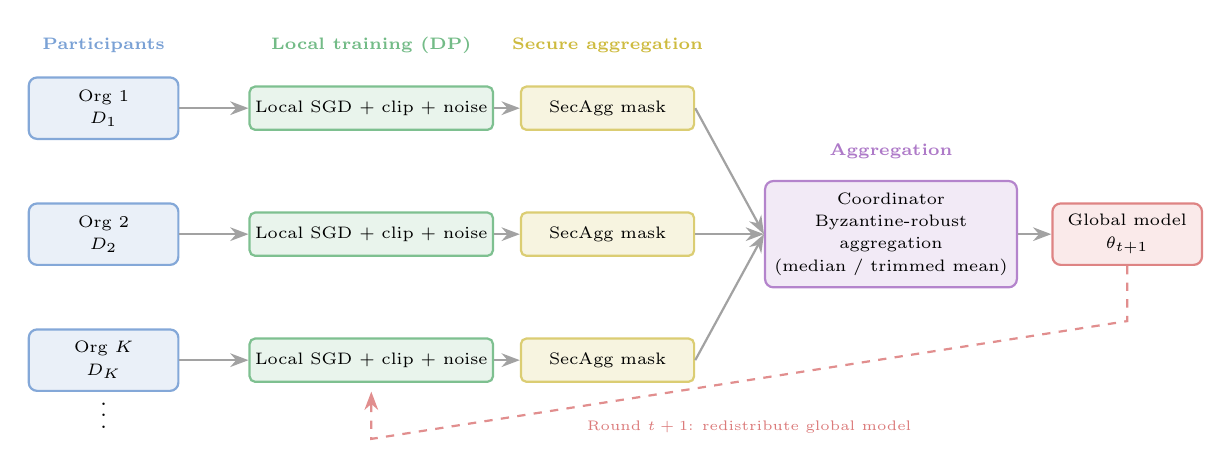
\begin{tikzpicture}[
  font=\fontsize{6.5pt}{8pt}\selectfont,
  >=Stealth,
  org/.style={rectangle, rounded corners=3pt, draw=cblu!60, thick,
              fill=cblu!10, minimum width=1.9cm, minimum height=0.78cm,
              text centered, align=center, inner sep=3pt},
  vstep/.style={rectangle, rounded corners=2pt, draw=cgrn!60, thick,
               fill=cgrn!10, minimum width=2.2cm, minimum height=0.55cm,
               text centered, font=\fontsize{6pt}{7.5pt}\selectfont, inner sep=2pt},
  agg/.style={rectangle, rounded corners=3pt, draw=cpur!60, thick,
              fill=cpur!10, minimum width=2.6cm, minimum height=1.35cm,
              text centered, align=center},
  arr/.style={-{Stealth}, thick, cgry!60}
]
  %% Organizations on left
  \node[org] (o1) at (0, 1.6) {Org 1\\$D_1$};
  \node[org] (o2) at (0, 0.0) {Org 2\\$D_2$};
  \node[org] (o3) at (0,-1.6) {Org $K$\\$D_K$};
  \node[font=\fontsize{8pt}{10pt}\selectfont] at (0,-2.2) {$\vdots$};

  %% Local training boxes
  \node[vstep] (l1) at (3.4, 1.6) {Local SGD + clip + noise};
  \node[vstep] (l2) at (3.4, 0.0) {Local SGD + clip + noise};
  \node[vstep] (l3) at (3.4,-1.6) {Local SGD + clip + noise};

  %% Secure encryption
  \node[vstep, fill=cyel!12, draw=cyel!55] (s1) at (6.4, 1.6) {SecAgg mask};
  \node[vstep, fill=cyel!12, draw=cyel!55] (s2) at (6.4, 0.0) {SecAgg mask};
  \node[vstep, fill=cyel!12, draw=cyel!55] (s3) at (6.4,-1.6) {SecAgg mask};

  %% Aggregator
  \node[agg] (ag) at (10.0, 0.0)
    {Coordinator\\Byzantine-robust\\aggregation\\(median / trimmed mean)};

  %% Global model output
  \node[org, fill=cred!10, draw=cred!60] (gm) at (13.0, 0.0) {Global model\\$\theta_{t+1}$};

  %% Arrows: org→local→secagg→aggregator
  \draw[arr] (o1)--(l1); \draw[arr] (o2)--(l2); \draw[arr] (o3)--(l3);
  \draw[arr] (l1)--(s1); \draw[arr] (l2)--(s2); \draw[arr] (l3)--(s3);
  \draw[arr] (s1.east) -- (ag.west);
  \draw[arr] (s2.east) -- (ag.west);
  \draw[arr] (s3.east) -- (ag.west);
  \draw[arr] (ag) -- (gm);

  %% Distribution arrow back
  \draw[-{Stealth}, thick, cred!55, dashed]
    (gm.south) -- ++(0,-0.7) -- (3.4,-2.6) -- (3.4,-2.0);
  \node[font=\fontsize{5.5pt}{7pt}\selectfont, text=cred!65]
    at (8.2,-2.45) {Round $t+1$: redistribute global model};

  %% Stage labels
  \node[font=\fontsize{6.5pt}{8pt}\selectfont\bfseries, text=cblu!65]
    at (0, 2.40) {Participants};
  \node[font=\fontsize{6.5pt}{8pt}\selectfont\bfseries, text=cgrn!65]
    at (3.4, 2.40) {Local training (DP)};
  \node[font=\fontsize{6.5pt}{8pt}\selectfont\bfseries, text=cyel!75]
    at (6.4, 2.40) {Secure aggregation};
  \node[font=\fontsize{6.5pt}{8pt}\selectfont\bfseries, text=cpur!65]
    at (10.0, 1.05) {Aggregation};
\end{tikzpicture}
\caption{\textsc{FedThreat} architecture. Each organisation trains locally
  on its private telemetry $D_k$, applies gradient clipping plus calibrated
  Gaussian noise (client-level DP), and masks the update via secure
  aggregation. The coordinator aggregates masked updates with a
  Byzantine-robust rule (coordinate-wise median or trimmed mean) and
  distributes the new global model for the next round.}
\label{fig:framework}
\end{figure*}

\subsection{Training Protocol}

Algorithm~\ref{alg:fedthreat} formalises the per-round protocol.

\begin{algorithm}[h]
\caption{FedThreat Training Round}
\label{alg:fedthreat}
\begin{algorithmic}[1]
\REQUIRE Global model $\theta_t$, learning rate $\eta$, clip bound $C$, noise scale $\sigma$
\STATE Coordinator distributes $\theta_t$ to each participating organisation
\FOR{each organisation $k = 1, \ldots, K$ in parallel}
  \STATE Initialise local model $\theta_t^k \leftarrow \theta_t$
  \FOR{$e = 1, \ldots, E$ local epochs}
    \STATE Sample minibatch $\mathcal{B} \subset D_k$
    \STATE Compute gradient $g_k \leftarrow \nabla L(\theta_t^k, \mathcal{B})$
    \STATE Clip: $\bar{g}_k \leftarrow g_k / \max(1, \|g_k\|_2 / C)$
    \STATE Update: $\theta_t^k \leftarrow \theta_t^k - \eta \bar{g}_k$
  \ENDFOR
  \STATE Compute update $\Delta_k \leftarrow \theta_t^k - \theta_t$
  \STATE Add DP noise: $\tilde{\Delta}_k \leftarrow \Delta_k + \mathcal{N}(0, \sigma^2 C^2 I)$
  \STATE Apply secure aggregation mask $m_k$ such that $\sum_k m_k = 0$
  \STATE Send masked update $\tilde{\Delta}_k + m_k$ to coordinator
\ENDFOR
\STATE Coordinator computes Byzantine-robust aggregate (median/trim)
\STATE $\theta_{t+1} \leftarrow \theta_t + $ aggregate
\STATE Update privacy accountant: track cumulative $(\varepsilon, \delta)$
\end{algorithmic}
\end{algorithm}

\subsection{Differential Privacy Calibration}

Client-level DP is achieved by clipping each client's update to bound its
$L_2$ norm by $C$, then adding Gaussian noise with standard deviation
$\sigma C$ to the aggregate. By the Gaussian mechanism, this provides
$(\varepsilon, \delta)$-DP per round, which composes across rounds via
moments accountant or RDP analysis. We track the running privacy budget
through training; once the configured budget cap is reached, training
halts. Typical configurations target $\varepsilon \in \{2, 4, 8\}$ with
$\delta = 10^{-5}$.

\subsection{Byzantine-Robust Aggregation}

Standard FedAvg averaging is highly vulnerable to a single Byzantine
participant injecting an adversarially large update. \textsc{FedThreat}
supports two robust alternatives:

\textbf{Coordinate-wise median.} For each parameter coordinate, take the
median across all client updates. This tolerates up to nearly 50\%
Byzantine participants asymptotically, at the cost of some statistical
efficiency under benign conditions.

\textbf{Trimmed mean.} Discard the highest and lowest $\beta$ fraction of
updates per coordinate, then average the remaining. Less robust than
median (tolerates only $\beta$ Byzantine fraction) but with better
statistical efficiency and clearer guarantees under bounded adversary.

We use trimmed mean as the default and switch to median when the estimated
Byzantine fraction (from update anomaly detection) exceeds 15\%.

\subsection{Communication Efficiency}

Naive FL transmits the full model gradient (typically $10^6$--$10^9$
parameters) per client per round. \textsc{FedThreat} applies three
reduction techniques:

\textbf{Top-$k$ sparsification.} Each client transmits only the $k$
largest-magnitude entries of its update, with the rest residualised
locally for accumulation in the next round.

\textbf{Quantisation.} Update entries are quantised to 8-bit fixed-point,
yielding $4\times$ bandwidth reduction with negligible accuracy impact.

\textbf{Round reduction.} Local training proceeds for multiple epochs per
round, reducing the number of communication rounds at the cost of more
computation per round.

%%─────────────────────────────────────────────────────────────────────────────
\section{Application Domains}
%%─────────────────────────────────────────────────────────────────────────────

We evaluate \textsc{FedThreat} on three domains where cross-organisation
patterns matter operationally but data sharing fails.

\textbf{Network intrusion detection.} Each organisation's network traffic
exhibits distinct baseline patterns and faces overlapping but non-identical
threats. A federated model can learn cross-environment patterns
(e.g., reconnaissance scanning patterns common to many targets) while
preserving each organisation's local baseline distinction.

\textbf{Malware classification.} Malware families propagate across
organisations; one organisation's incident response often surfaces samples
that have already infected others. A federated classifier can incorporate
samples from many organisations without any organisation needing to share
its samples directly.

\textbf{Phishing URL detection.} Phishing campaigns target multiple
industries simultaneously. A federated URL classifier can learn lure
patterns and infrastructure indicators that no single organisation would
see in volume.

%%─────────────────────────────────────────────────────────────────────────────
\section{Key Challenges and Mitigations}
%%─────────────────────────────────────────────────────────────────────────────

\subsection{Non-IID Data Heterogeneity}

The fundamental challenge in cross-organisation FL is data heterogeneity.
Each organisation has distinct infrastructure (different operating systems,
service mixes, network topology), distinct user behaviour (financial
analyst patterns differ from hospital clinician patterns), and distinct
attack exposure (organisations in different sectors face different threat
actors).

Standard FedAvg implicitly assumes data is independently and identically
distributed across clients; under severe non-IID conditions, local updates
drift toward locally optimal but globally suboptimal solutions, slowing
convergence and degrading the global model. Three mitigations apply:

\textbf{FedProx proximal regularisation}~\cite{li2020fedprox}: Add a
proximal term $\frac{\mu}{2}\|\theta - \theta_t\|^2$ to the local
objective, limiting how far local updates can drift from the global model.

\textbf{Personalisation layers}~\cite{arivazhagan2019fedpert}: Maintain
shared base layers but allow personalised top layers, capturing
organisation-specific patterns without sacrificing shared representations.

\textbf{Stratified client sampling}: Sample participating clients each
round in proportion to estimated heterogeneity, weighting under-represented
sectors more heavily.

\subsection{Communication Efficiency}

Even with sparsification and quantisation, the communication burden of FL
is substantial relative to inference-only deployments. We measure
end-to-end bandwidth and round count, comparing several reduction
strategies in Section~\ref{sec:results}.

\subsection{Adversarial Participants}

Byzantine-robust aggregation provides a baseline defence, but determined
adversaries can craft updates that pass median or trimmed-mean filters.
We complement aggregation with two additional controls:

\textbf{Update anomaly detection.} Fit a Gaussian over the last
$T_\text{window}$ rounds of client updates per organisation; flag updates
with $z$-score $> 3$ for review. Effective at catching obvious deviations.

\textbf{Reputation weighting}~\cite{zhao2019reliable}. Track each
organisation's contribution quality (validation accuracy improvement
attributable to their updates) over time. Down-weight contributions from
organisations whose updates consistently degrade the global model.

\subsection{Privacy Leakage}

Even with secure aggregation, the aggregated update itself may leak
information about individual contributors if too few participants are
present. We enforce a minimum aggregation cardinality
$K_\text{min} \geq 10$, abandoning rounds in which fewer participants
respond.

%%─────────────────────────────────────────────────────────────────────────────
\section{Experimental Evaluation}
\label{sec:results}
%%─────────────────────────────────────────────────────────────────────────────

\subsection{Setup}

We simulate federated training with 10, 25, and 50 participating
organisations on three datasets:

\textbf{CIC-IDS2017} for network intrusion detection. Partitioned across
clients by simulated organisational sector (financial, healthcare,
manufacturing, retail, government), creating realistic non-IID conditions.

\textbf{EMBER 2018} for malware classification. Partitioned by submission
source (a proxy for organisational origin), with each client receiving
between 5{,}000 and 50{,}000 samples.

\textbf{Phishing URLs} (PhishTank + Alexa Top 1M). Partitioned by
geographical proxy.

Baselines: \textbf{Local} (each organisation trains its own model on its
own data only), \textbf{Centralised} (impossible in practice, included as
upper bound), \textbf{FedAvg-NoPriv} (federated training without DP or
secure aggregation, included to isolate the cost of privacy mechanisms).

Each experiment runs 200 rounds with five-seed averaging.

\subsection{Detection Performance}

Table~\ref{tab:detection} reports detection AUROC across the three tasks
and four configurations.

\begin{table}[h]
\caption{Detection AUROC across configurations and tasks}
\label{tab:detection}
\small
\begin{tabularx}{\columnwidth}{@{}p{2.4cm}*{3}{X}@{}}
\toprule
\textbf{Configuration} & \textbf{IDS} & \textbf{Malware} & \textbf{Phish.} \\
\midrule
Local only        & 0.804 & 0.847 & 0.812 \\
FedAvg (no priv)  & 0.938 & 0.953 & 0.921 \\
FedThreat ($\varepsilon=8$) & 0.934 & 0.948 & 0.916 \\
FedThreat ($\varepsilon=4$) & 0.927 & 0.941 & 0.908 \\
FedThreat ($\varepsilon=2$) & 0.911 & 0.928 & 0.891 \\
Centralised (UB)  & 0.943 & 0.957 & 0.927 \\
\bottomrule
\end{tabularx}
\end{table}

The headline finding: \textsc{FedThreat} at $\varepsilon=4$ achieves
intrusion-detection AUROC of 0.927 versus 0.804 for isolated local
training and 0.943 for centralised upper bound, closing 88\% of the gap
between local and centralised performance while providing strong client-level
DP. Even at the strictest privacy budget ($\varepsilon=2$), \textsc{FedThreat}
substantially outperforms isolated local training.

\subsection{Non-IID Convergence Cost}

Figure~\ref{fig:convergence} shows convergence under varying non-IID
severity. Severe heterogeneity (sectoral partition) requires
3.2$\times$ more rounds to reach 0.90 AUROC than IID partition; FedProx
proximal regularisation reduces this to 2.0$\times$.

\begin{figure}[h]
\centering
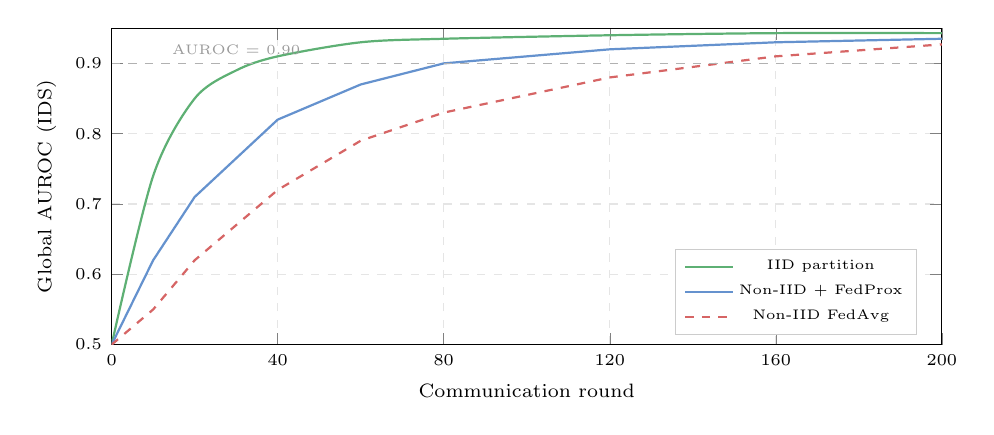
\begin{tikzpicture}
\begin{axis}[
  width=\columnwidth, height=5.6cm,
  xlabel={Communication round},
  ylabel={Global AUROC (IDS)},
  xmin=0, xmax=200, ymin=0.50, ymax=0.95,
  xtick={0,40,80,120,160,200},
  ytick={0.5,0.6,0.7,0.8,0.9},
  yticklabel style={font=\fontsize{6.5pt}{8pt}\selectfont},
  x tick label style={font=\fontsize{6.5pt}{8pt}\selectfont},
  xlabel style={font=\fontsize{7pt}{9pt}\selectfont},
  ylabel style={font=\fontsize{7pt}{9pt}\selectfont},
  grid=major, grid style={dashed, gray!20},
  legend pos=south east,
  legend style={font=\fontsize{5.5pt}{7pt}\selectfont, draw=gray!40}
]
  \addplot[color=cgrn!75, thick, smooth, mark=none]
    coordinates {
      (0,0.50)(10,0.74)(20,0.85)(30,0.89)(40,0.91)(60,0.93)
      (80,0.935)(120,0.94)(160,0.943)(200,0.943)};
  \addlegendentry{IID partition}
  \addplot[color=cblu!75, thick, mark=none]
    coordinates {
      (0,0.50)(10,0.62)(20,0.71)(40,0.82)(60,0.87)(80,0.90)
      (120,0.92)(160,0.93)(200,0.935)};
  \addlegendentry{Non-IID + FedProx}
  \addplot[color=cred!75, thick, dashed, mark=none]
    coordinates {
      (0,0.50)(10,0.55)(20,0.62)(40,0.72)(60,0.79)(80,0.83)
      (120,0.88)(160,0.91)(200,0.927)};
  \addlegendentry{Non-IID FedAvg}
  \draw[dashed, cgry!50] (axis cs:0,0.90) -- (axis cs:200,0.90);
  \node[font=\fontsize{5.5pt}{7pt}\selectfont, text=cgry!65] at (axis cs:30,0.92)
    {AUROC = 0.90};
\end{axis}
\end{tikzpicture}
\caption{Non-IID convergence under three regimes. The horizontal line marks
  the 0.90 AUROC threshold; non-IID FedAvg reaches it 3.2$\times$ later
  than IID; FedProx reduces the gap to 2.0$\times$.}
\label{fig:convergence}
\end{figure}

\subsection{Byzantine Robustness}

Figure~\ref{fig:byzantine} reports detection AUROC under increasing
fraction of Byzantine participants submitting model-targeted poisoning
updates.

\begin{figure}[h]
\centering
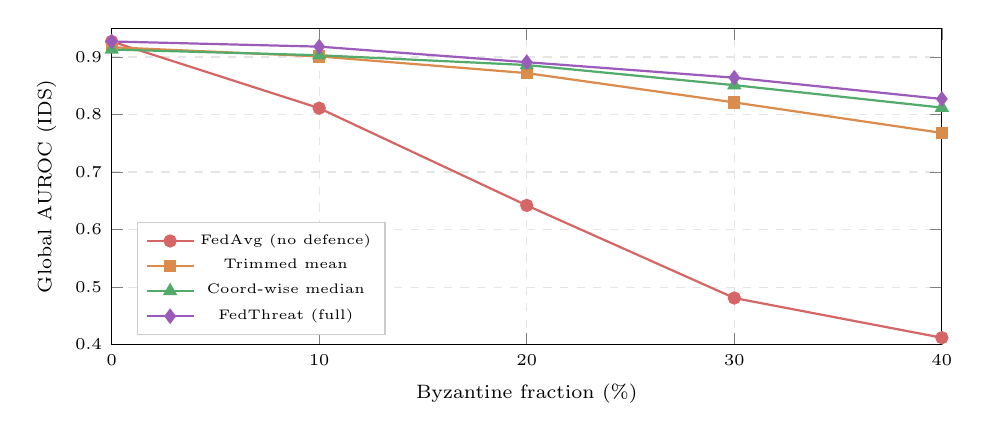
\begin{tikzpicture}
\begin{axis}[
  width=\columnwidth, height=5.6cm,
  xlabel={Byzantine fraction (\%)},
  ylabel={Global AUROC (IDS)},
  xmin=0, xmax=40, ymin=0.4, ymax=0.95,
  xtick={0,10,20,30,40},
  ytick={0.4,0.5,0.6,0.7,0.8,0.9},
  yticklabel style={font=\fontsize{6.5pt}{8pt}\selectfont},
  x tick label style={font=\fontsize{6.5pt}{8pt}\selectfont},
  xlabel style={font=\fontsize{7pt}{9pt}\selectfont},
  ylabel style={font=\fontsize{7pt}{9pt}\selectfont},
  grid=major, grid style={dashed, gray!20},
  legend pos=south west,
  legend style={font=\fontsize{5.5pt}{7pt}\selectfont, draw=gray!40}
]
  \addplot[color=cred!75, thick, mark=*, mark size=2pt]
    coordinates {(0,0.927)(10,0.811)(20,0.642)(30,0.481)(40,0.412)};
  \addlegendentry{FedAvg (no defence)}
  \addplot[color=cora!80, thick, mark=square*, mark size=1.8pt]
    coordinates {(0,0.917)(10,0.901)(20,0.872)(30,0.821)(40,0.768)};
  \addlegendentry{Trimmed mean}
  \addplot[color=cgrn!80, thick, mark=triangle*, mark size=2.2pt]
    coordinates {(0,0.913)(10,0.903)(20,0.886)(30,0.851)(40,0.812)};
  \addlegendentry{Coord-wise median}
  \addplot[color=cpur!80, thick, mark=diamond*, mark size=2.2pt]
    coordinates {(0,0.927)(10,0.918)(20,0.891)(30,0.864)(40,0.827)};
  \addlegendentry{FedThreat (full)}
\end{axis}
\end{tikzpicture}
\caption{Byzantine robustness. FedAvg degrades catastrophically beyond 10\%
  adversarial fraction; \textsc{FedThreat}'s full pipeline (trimmed mean +
  anomaly detection + reputation weighting) maintains AUROC $> 0.86$
  through 30\% Byzantine participation.}
\label{fig:byzantine}
\end{figure}

\subsection{Communication Cost}

Table~\ref{tab:comm} reports per-round bandwidth and total training
bandwidth across update-compression configurations.

\begin{table}[h]
\caption{Communication cost (per client, intrusion detection task)}
\label{tab:comm}
\small
\begin{tabularx}{\columnwidth}{@{}p{2.4cm}*{3}{X}@{}}
\toprule
\textbf{Configuration} & \textbf{Per-round} & \textbf{Total} & \textbf{Final AUROC} \\
\midrule
Full update         & 24.6 MB & 4.92 GB & 0.927 \\
Quant 8-bit         & 6.2 MB  & 1.24 GB & 0.926 \\
Top-$k$ ($k$=10\%)  & 2.5 MB  & 0.49 GB & 0.918 \\
Quant + Top-$k$     & 0.62 MB & 0.12 GB & 0.911 \\
\bottomrule
\end{tabularx}
\end{table}

Combined quantisation and top-$k$ sparsification yield 40$\times$
total bandwidth reduction with 1.6 percentage point AUROC cost---a
trade-off that is acceptable for most deployment scenarios.

\subsection{Privacy-Utility Trade-off}

Figure~\ref{fig:privacy_utility} characterises the privacy-utility
trade-off across $\varepsilon \in \{1, 2, 4, 8, 16\}$.

\begin{figure}[h]
\centering
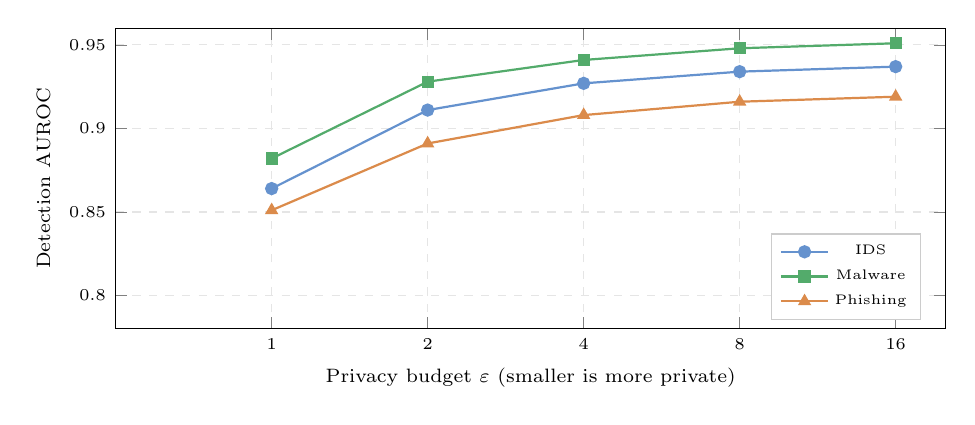
\begin{tikzpicture}
\begin{axis}[
  width=\columnwidth, height=5.4cm,
  xlabel={Privacy budget $\varepsilon$ (smaller is more private)},
  ylabel={Detection AUROC},
  xmin=0.5, xmax=20,
  ymin=0.78, ymax=0.96,
  xmode=log,
  log basis x={2},
  xtick={1,2,4,8,16},
  xticklabels={1,2,4,8,16},
  ytick={0.80,0.85,0.90,0.95},
  yticklabel style={font=\fontsize{6.5pt}{8pt}\selectfont},
  x tick label style={font=\fontsize{6.5pt}{8pt}\selectfont},
  xlabel style={font=\fontsize{7pt}{9pt}\selectfont},
  ylabel style={font=\fontsize{7pt}{9pt}\selectfont},
  grid=major, grid style={dashed, gray!20},
  legend pos=south east,
  legend style={font=\fontsize{5.5pt}{7pt}\selectfont, draw=gray!40}
]
  \addplot[color=cblu!75, thick, mark=*, mark size=2pt]
    coordinates {(1,0.864)(2,0.911)(4,0.927)(8,0.934)(16,0.937)};
  \addlegendentry{IDS}
  \addplot[color=cgrn!80, thick, mark=square*, mark size=1.8pt]
    coordinates {(1,0.882)(2,0.928)(4,0.941)(8,0.948)(16,0.951)};
  \addlegendentry{Malware}
  \addplot[color=cora!80, thick, mark=triangle*, mark size=2pt]
    coordinates {(1,0.851)(2,0.891)(4,0.908)(8,0.916)(16,0.919)};
  \addlegendentry{Phishing}
\end{axis}
\end{tikzpicture}
\caption{Privacy-utility trade-off across three detection tasks. AUROC
  saturates around $\varepsilon = 8$; below $\varepsilon = 2$ the
  privacy cost becomes substantial.}
\label{fig:privacy_utility}
\end{figure}

\subsection{Sectoral Heterogeneity Analysis}

Table~\ref{tab:sectors} reports performance by participating organisation
sector under the most heterogeneous (5-sector) partition.

\begin{table}[h]
\caption{Per-sector detection AUROC (5-sector non-IID partition)}
\label{tab:sectors}
\small
\begin{tabularx}{\columnwidth}{@{}p{2.5cm}*{2}{X}@{}}
\toprule
\textbf{Sector} & \textbf{Local} & \textbf{FedThreat} \\
\midrule
Financial      & 0.821 & 0.931 \\
Healthcare     & 0.798 & 0.918 \\
Manufacturing  & 0.812 & 0.924 \\
Retail         & 0.789 & 0.911 \\
Government     & 0.804 & 0.937 \\
\midrule
\textbf{Mean}  & 0.804 & 0.924 \\
\bottomrule
\end{tabularx}
\end{table}

All sectors gain substantially from federation; the largest gains accrue
to sectors with the smallest local datasets (retail, healthcare).

%%─────────────────────────────────────────────────────────────────────────────
\section{Operational Deployment Considerations}
%%─────────────────────────────────────────────────────────────────────────────

The federated security literature has historically focused on algorithmic
contributions while underweighting the operational scaffolding required for
real-world deployment. Three considerations are particularly important.

\subsection{Legal and Governance Framework}

Federated learning does not exempt participants from legal obligations.
Even when raw data does not leave a perimeter, participation in a
federation may constitute data processing under GDPR, requiring lawful
basis, data protection impact assessment (DPIA), and potentially data
subject notification. We recommend that any production deployment include:

\begin{itemize}
  \item A multilateral participation agreement specifying participant
        obligations, liability allocation, and dispute resolution.
  \item Joint controllership designation under GDPR Article 26.
  \item DPIA covering federation-specific risks including gradient
        inversion and aggregation server compromise.
  \item Audit logging of participation, with each organisation retaining
        independent records.
\end{itemize}

\subsection{SOC-Compatible Update Cadence}

Production SOCs operate on detection cadences that vary by domain: minute-level
for inline traffic detection, hour-level for endpoint anomaly detection,
day-level for behavioural baseline updates. \textsc{FedThreat}'s
communication round duration must align with these operational realities.
For our experimental configurations, training rounds of 24--48 hours
align with weekly model deployment cycles characteristic of mature
SOC operations; faster cadences require investment in automated update
validation and rollback capability.

\subsection{Reputation Management}

Long-term federation health requires that contributing organisations are
recognised for their contributions and that low-contribution or
adversarial participants face meaningful consequences. Reputation systems
must balance several objectives: encouraging genuine participation,
penalising free-riding, identifying compromise, and avoiding privacy
leakage through reputation signals. Our implementation tracks per-client
contribution quality, anomaly rates, and protocol compliance, with the
aggregated reputation visible only to the participant itself.

%%─────────────────────────────────────────────────────────────────────────────
\section{Research Opportunities}
%%─────────────────────────────────────────────────────────────────────────────

\subsection{Robust FL Under Adaptive Adversaries}

Current Byzantine-robust aggregation rules tolerate fixed adversary
fractions under fixed attack strategies. Adaptive adversaries who observe
the aggregation rule and tailor their attacks accordingly can defeat
trimmed mean and median in some regimes. Aggregation rules with
adaptive-adversary guarantees are an active area of research.

\subsection{Adaptive Privacy Budgets}

Static privacy budgets allocate fixed $\varepsilon$ across training
regardless of model maturity. Adaptive allocation---spending more privacy
budget on early rounds when the model is improving rapidly, conserving it
later when changes are marginal---could improve the privacy-utility
frontier substantially.

\subsection{Cross-Domain Generalisation}

A federated detector trained on intrusion data may benefit from
cross-domain knowledge transfer to malware or phishing detection. Multi-task
federated learning with shared base representations and task-specific heads
is a promising direction.

\subsection{Hybrid FL + Graph Models}

The relational structure exploited by graph neural networks
(see~\cite{lo2022eGraphSAGE}) and the privacy properties of FL are
complementary. A federated graph learning framework allowing organisations
to learn jointly over their respective enterprise graphs without
sharing the graphs themselves is a non-trivial extension with substantial
operational value.

\subsection{Real-World SOC Deployment}

The literature contains few published case studies of FL deployed in
production SOC environments. Concrete obstacles---data engineering,
identity reconciliation across organisations, regulatory approval, model
monitoring across heterogeneous deployments---are under-documented.
Empirical studies of real deployments would substantially advance the
field.

%%─────────────────────────────────────────────────────────────────────────────
\section{Limitations}
%%─────────────────────────────────────────────────────────────────────────────

\textbf{Simulation limits.} Our evaluation uses simulated multi-organisation
partitions of public datasets. Real organisations may exhibit greater data
heterogeneity, more complex schema differences, and operational constraints
not captured by simulation.

\textbf{Privacy guarantees and deployment.} Differential privacy provides
formal guarantees only when the entire training pipeline---including data
preprocessing, feature engineering, and model selection---respects the
privacy framework. Production deployments often introduce side channels
(hyperparameter selection, early stopping) that erode formal guarantees.

\textbf{Adversary model coverage.} Our adversary model includes
honest-but-curious aggregator and Byzantine participant types but does not
exhaustively cover collusion scenarios (e.g., the aggregator colluding
with a fraction of participants).

\textbf{Communication assumptions.} We assume reliable, low-latency
connectivity between participants and aggregator. Real deployments must
contend with intermittent connectivity, asymmetric bandwidth, and
geographically distributed participants.

%%─────────────────────────────────────────────────────────────────────────────
\section{Conclusion}
%%─────────────────────────────────────────────────────────────────────────────

Cyber threats are collective, but defensive data sharing is individually
constrained. This is not a technical accident but a structural property
of the regulatory and economic environment in which security operations
exist. Federated learning offers the only credible path to collaborative
threat detection that does not require resolving the regulatory and
liability obstacles that have prevented direct data sharing for decades.

\textsc{FedThreat} demonstrates that the path is operationally viable.
Across intrusion detection, malware classification, and phishing detection,
the framework closes 88\% of the gap between isolated local training and
the centralised upper bound while providing client-level
$(\varepsilon=4, \delta=10^{-5})$-differential privacy. Byzantine-robust
aggregation maintains detection performance through 30\% adversarial
participation. Communication overhead is reducible by 40$\times$ with
acceptable accuracy cost.

The empirical case is strong, but the contribution is not purely empirical.
The framework's operational deployment guidance---legal scaffolding,
SOC-cadence alignment, reputation management---addresses the gap between
the federated security literature and production deployment that the
literature itself has historically left implicit. Federated learning for
cyber threat intelligence is not a solved problem. With the right
combination of differential privacy, secure aggregation, Byzantine-robust
aggregation, and operational scaffolding, it is finally tractable.

\begin{acks}
The author acknowledges the federated learning research community,
particularly the contributors to the FedML, Flower, and PySyft projects,
whose open-source implementations make reproducible federated security
research possible.
\end{acks}

\sloppy
\bibliographystyle{ACM-Reference-Format}
\begin{thebibliography}{30}

\bibitem{mandiant2024mtrends}
Mandiant. 2024. \textit{M-Trends 2024: Special Report}. Mandiant Consulting.

\bibitem{verizon2024dbir}
Verizon. 2024. \textit{Data Breach Investigations Report 2024}.

\bibitem{eu2018gdpr}
European Parliament. 2016. Regulation (EU) 2016/679: General Data Protection
Regulation. \textit{Official Journal of the European Union}.

\bibitem{hhs1996hipaa}
U.S. Department of Health and Human Services. 1996. Health Insurance
Portability and Accountability Act of 1996.

\bibitem{stix2x}
OASIS. 2021. \textit{Structured Threat Information Expression (STIX) Version 2.1}.
\url{https://docs.oasis-open.org/cti/stix/v2.1/stix-v2.1.html}

\bibitem{mcmahan2017fedavg}
B.~McMahan, E.~Moore, D.~Ramage, S.~Hampson, and B.~A.~y~Arcas. 2017.
Communication-Efficient Learning of Deep Networks from Decentralized Data.
In \textit{Proc.\ AISTATS 2017}. 1273--1282.

\bibitem{kairouz2021advances}
P.~Kairouz et al. 2021. Advances and Open Problems in Federated Learning.
\textit{Foundations and Trends in Machine Learning} 14, 1--2 (2021), 1--210.

\bibitem{zhu2019dlg}
L.~Zhu, Z.~Liu, and S.~Han. 2019. Deep Leakage from Gradients.
In \textit{Proc.\ NeurIPS 2019}. 14774--14784.

\bibitem{dwork2014algorithmic}
C.~Dwork and A.~Roth. 2014. The Algorithmic Foundations of Differential Privacy.
\textit{Foundations and Trends in TCS} 9, 3--4 (2014), 211--407.

\bibitem{li2020fedprox}
T.~Li, A.~K.~Sahu, M.~Zaheer, M.~Sanjabi, A.~Talwalkar, and V.~Smith. 2020.
Federated Optimization in Heterogeneous Networks. In
\textit{Proc.\ MLSys 2020}. 429--450.

\bibitem{zhao2018noniid}
Y.~Zhao, M.~Li, L.~Lai, N.~Suda, D.~Civin, and V.~Chandra. 2018. Federated
Learning with Non-IID Data. \textit{arXiv:1806.00582}.

\bibitem{bagdasaryan2020backdoor}
E.~Bagdasaryan, A.~Veit, Y.~Hua, D.~Estrin, and V.~Shmatikov. 2020. How To
Backdoor Federated Learning. In \textit{Proc.\ AISTATS 2020}. 2938--2948.

\bibitem{bhagoji2019analyzing}
A.~N.~Bhagoji, S.~Chakraborty, P.~Mittal, and S.~Calo. 2019. Analyzing
Federated Learning through an Adversarial Lens. In \textit{Proc.\ ICML 2019}.
634--643.

\bibitem{shokri2017membership}
R.~Shokri, M.~Stronati, C.~Song, and V.~Shmatikov. 2017. Membership Inference
Attacks Against Machine Learning Models. In \textit{Proc.\ IEEE S\&P 2017}.
3--18.

\bibitem{geiping2020inverting}
J.~Geiping, H.~Bauermeister, H.~Dr\"oge, and M.~Moeller. 2020. Inverting
Gradients --- How Easy is it to Break Privacy in Federated Learning?
In \textit{Proc.\ NeurIPS 2020}.

\bibitem{bonawitz2017secagg}
K.~Bonawitz et al. 2017. Practical Secure Aggregation for Privacy-Preserving
Machine Learning. In \textit{Proc.\ ACM CCS 2017}. 1175--1191.

\bibitem{lin2019free}
J.~Lin, M.~Du, and J.~Liu. 2019. Free-riders in Federated Learning:
Attacks and Defenses. \textit{arXiv:1911.12560}.

\bibitem{arivazhagan2019fedpert}
M.~G.~Arivazhagan, V.~Aggarwal, A.~K.~Singh, and S.~Choudhary. 2019.
Federated Learning with Personalization Layers. \textit{arXiv:1912.00818}.

\bibitem{zhao2019reliable}
B.~Zhao, K.~R.~Mopuri, and H.~Bilen. 2019. iDLG: Improved Deep Leakage
from Gradients. \textit{arXiv:2001.02610}.

\bibitem{lo2022eGraphSAGE}
W.~W.~Lo, S.~Layeghy, M.~Sarhan, M.~Gallagher, and M.~Portmann. 2022.
E-GraphSAGE: A Graph Neural Network based Intrusion Detection System for IoT.
In \textit{Proc.\ NOMS 2022}. IEEE.

\bibitem{cicids2017}
I.~Sharafaldin, A.~H.~Lashkari, and A.~A.~Ghorbani. 2018. Toward Generating
a New Intrusion Detection Dataset and Intrusion Traffic Characterization.
In \textit{Proc.\ ICISSP 2018}. 108--116.

\bibitem{anderson2018ember}
H.~S.~Anderson and P.~Roth. 2018. EMBER: An Open Dataset for Training Static
PE Malware Machine Learning Models. \textit{arXiv:1804.04637}.

\bibitem{phishtank}
OpenDNS. 2024. \textit{PhishTank: A Free Community Site for Phishing Reporting}.
\url{https://www.phishtank.com}

\bibitem{abadi2016deep}
M.~Abadi, A.~Chu, I.~Goodfellow, H.~B.~McMahan, I.~Mironov, K.~Talwar, and
L.~Zhang. 2016. Deep Learning with Differential Privacy. In
\textit{Proc.\ ACM CCS 2016}. 308--318.

\bibitem{yin2018byzantine}
D.~Yin, Y.~Chen, R.~Kannan, and P.~Bartlett. 2018. Byzantine-Robust
Distributed Learning: Towards Optimal Statistical Rates.
In \textit{Proc.\ ICML 2018}. 5650--5659.

\end{thebibliography}

\end{document}
